 \subsubsection{2-Tore} \label{subsubsec:2tore}
  
2-Tore sind Netzwerke mit 2 Klemmenpaaren. Ein Klemmenpaar wird auch als Tor bezeichnet. Diese sind intern aus beliebigen R (ohmischer Widerstand), L (Induktivität), C (Kapazität) und M(Gegeninduktivität) Komponenten aufgebaut. Dabei wird ein Tor als Eingang für ein Elektrisches Signal verwendet. Folglich wird am Anderen Tor das Ausgangssignal abgegriffen. Es wird zwischen aktiven (Signal verstärkend) und passiven (Signal abschwächend) Zweitoren unterschieden. Eine einfache Methode um 2-Tore zu berechnen ist die Kettenmatrix. 

\begin{figure}[H]
	\centering
	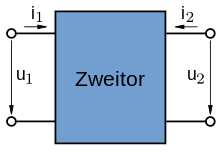
\includegraphics[width=5cm]{2Tor.png}
	\label{fig:2tor}
\end{figure}

Lineare 2-Tore sind zudem Reziprok. Reziprozität bedeutet, dass es egal ist, in welcher Richtung das Netzwerk betrieben wird, solange der Innenwiderstand der Quelle gleich gross ist wie  die Lastimpedanz.

\begin{figure}[H]
	\centering
	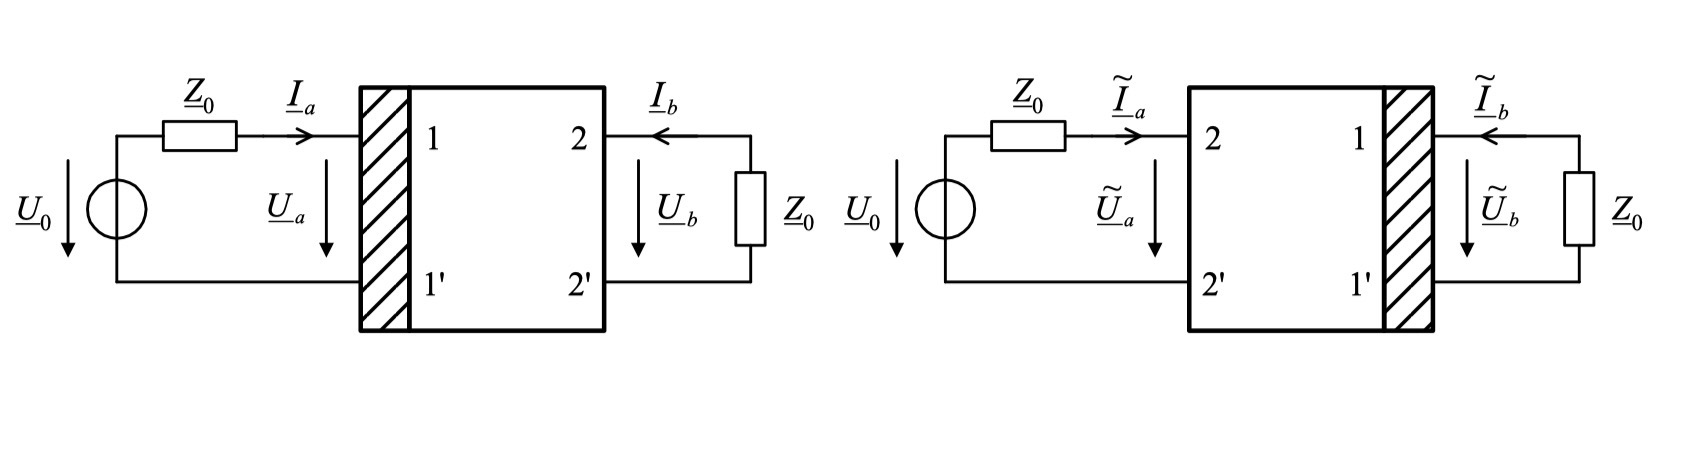
\includegraphics[width=12cm]{reziprozitat.jpg}
	\label{fig:reziprozitat}
\end{figure}

Im dargestellten Netzwerk gilt somit

\begin{equation}\label{equ:verticImpedance}
			\underline{I}_b =  \underline{\tilde{I}}_b
		\end{equation}
		
sowie 		
		
\begin{equation}\label{equ:verticImpedance}
			\underline{U}_b =  \underline{\widetilde{U}}_b
		\end{equation}
		
Die Reziprozität des Netzwerks sorgt für eine grosse Rechenerleichterung.
